% ═════════════════════════════════════════════════════════════════════════════
\appendix
\section{Appendix}
\label{sec:appendix}

% ─── A.1 Full EDA Plots ───────────────────────────────────────────────────────
\subsection{Full EDA Plots}

\begin{figure}[H]
  \centering
  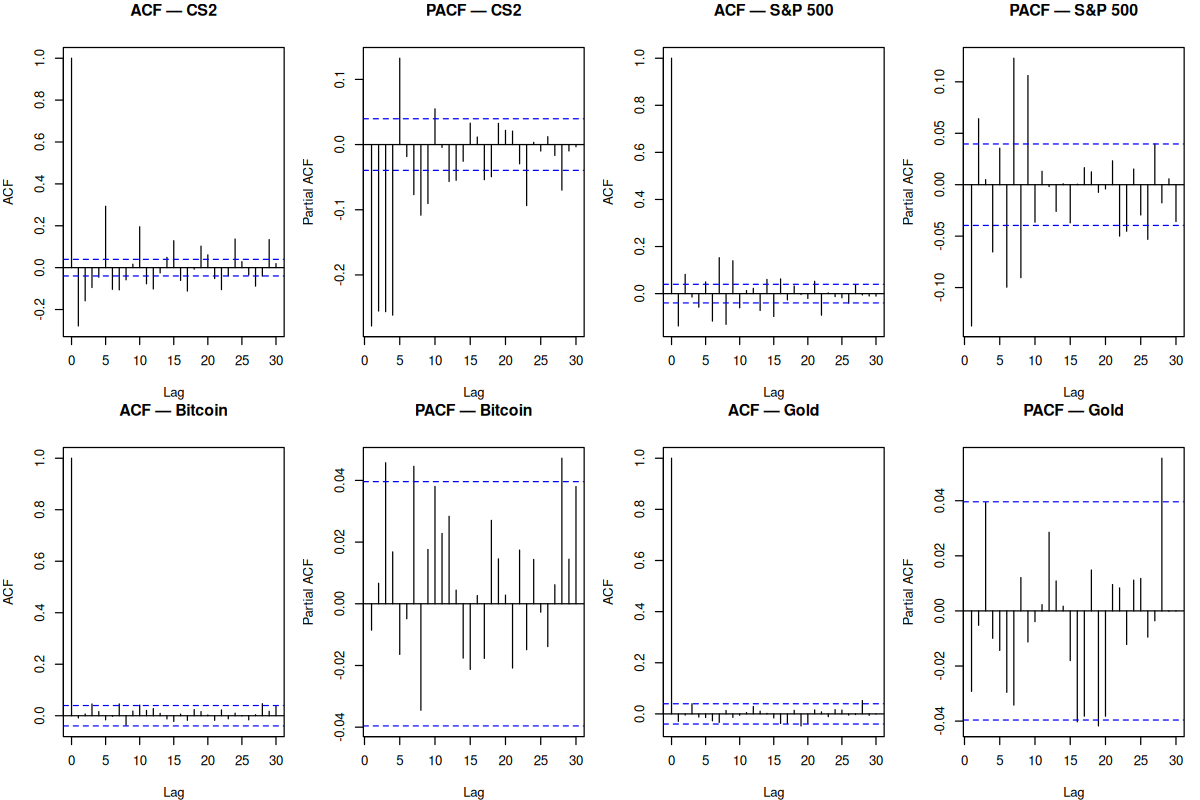
\includegraphics[width=\linewidth]{../images/eda/acf.png}
  \caption{Autocorrelation (ACF) and Partial Autocorrelation (PACF) of daily log
    returns for all four assets at up to 30 lags.}
  \label{fig:acf}
\end{figure}

The ACF plots confirm two key properties of the return series.
First, the ACF of log returns shows no significant linear autocorrelation at
any lag for any asset --- a necessary condition for the absence of exploitable
linear predictability in returns. (Note: the VAR(4) residuals for CS2 do
reveal remaining structure not visible in the raw ACF; see Table~\ref{tab:ljungbox}
for details.) Second, the ACF of squared returns reveals significant, slowly
decaying autocorrelation for all assets, a hallmark of ARCH effects and the
empirical motivation for the GARCH specification.
CS2 squared returns exhibit noticeably slower decay than Bitcoin and the
S\&P~500, indicating that CS2 volatility shocks persist in long regimes rather
than dissipating quickly --- consistent with the low ARCH coefficient
($\hat{\alpha} = 0.0151$) and high GARCH coefficient ($\hat{\beta} = 0.9839$)
estimated in Section~\ref{subsec:garch}.

\begin{figure}[H]
  \centering
  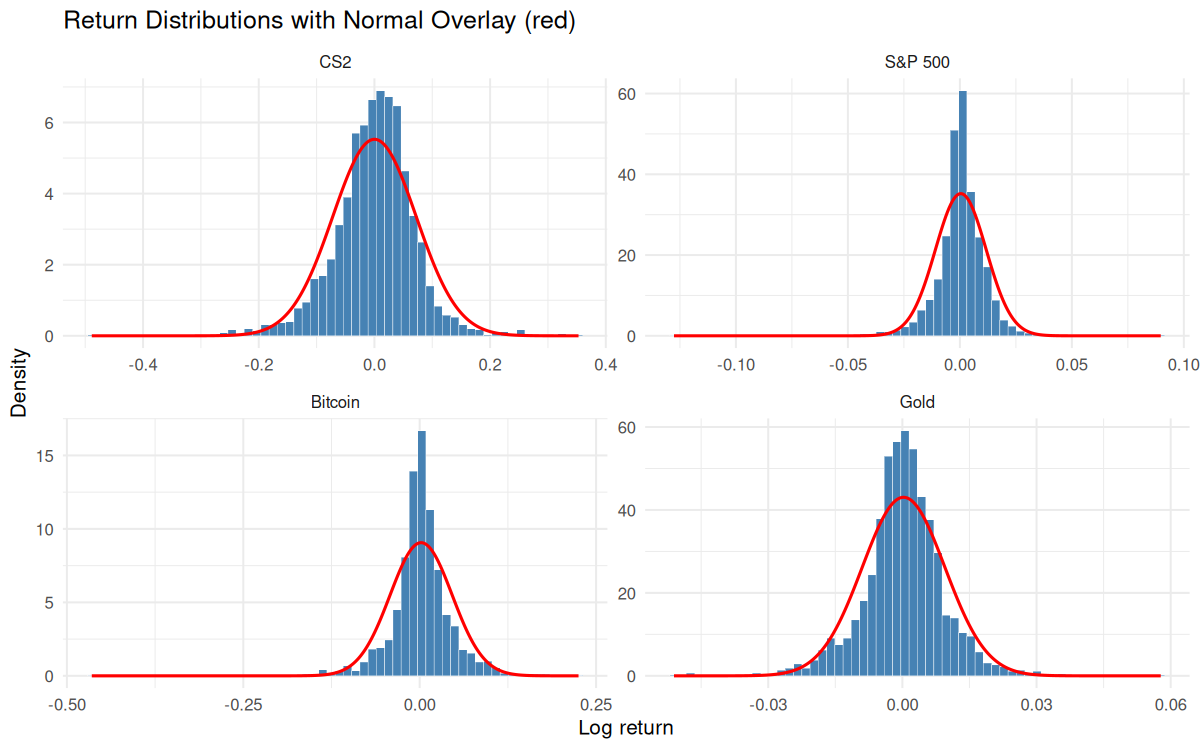
\includegraphics[width=\linewidth]{../images/eda/distributions.png}
  \caption{Empirical return distributions (histogram) overlaid with a fitted
    normal curve (red) for all four assets.}
  \label{fig:distributions}
\end{figure}

All four return series are leptokurtic, exhibiting fatter tails than the normal
distribution. The departure is most pronounced for the S\&P~500 (excess kurtosis
15.74) and Bitcoin (9.07), reflecting the high frequency of extreme return events
in both markets. CS2 shows moderate excess kurtosis (3.82), above that of Gold
(3.77), but below the two more liquid markets --- plausibly because the
Steam Marketplace's slow price-adjustment microstructure dampens extreme
one-day moves. The systematic fat-tail pattern across all assets confirms the
appropriateness of student-$t$ innovations in the GARCH specification (rather
than a Gaussian assumption), and the absence of a pronounced second mode in any
distribution rules out bimodality as a confound.

% ─── A.2 Index Construction Details ──────────────────────────────────────────
\subsection{Index Construction Details}

\begin{table}[H]
\centering
\caption{Item Filter Funnel --- CS2 Index Construction}
\label{tab:filter_funnel}
\begin{tabular}{lrr}
\hline
Stage & Item variants & Base items \\
\hline
Raw items (all categories, all variants) & 22{,}446 & 10{,}833 \\
After wearable + StatTrak/Souvenir filter & 7{,}348 & 1{,}638 \\
After liquidity filter ($\geq$2 trades/month) & --- & 1{,}607 \\
\hline
\end{tabular}
\end{table}

Table~\ref{tab:filter_funnel} documents the item reduction at each construction
stage. The raw dataset comprises 22,446 distinct item variants (combinations of
base item and wear condition) across 10,833 base items spanning all Steam
Marketplace categories. Restricting to wearable categories (weapon skins,
knives, gloves) and excluding StatTrak and Souvenir variants reduces the sample
to 7,348 item variants across 1,638 base items. This step removes items whose
prices are inflated by premium mechanics rather than driven by the underlying
cosmetic market, ensuring the index reflects comparable, freely-tradeable assets.
The final liquidity filter --- requiring at least two recorded transactions in
every calendar month --- removes a further 31 base items (2\%), retaining 1,607
items. The criterion is analogous to the SIX minimum turnover requirement for
equity index inclusion \cite{six2024indexcriteria}: items failing it trade too
infrequently for their daily prices to be reliable signals, and including them
would introduce stale-price bias into the index level.

\begin{figure}[H]
  \centering
  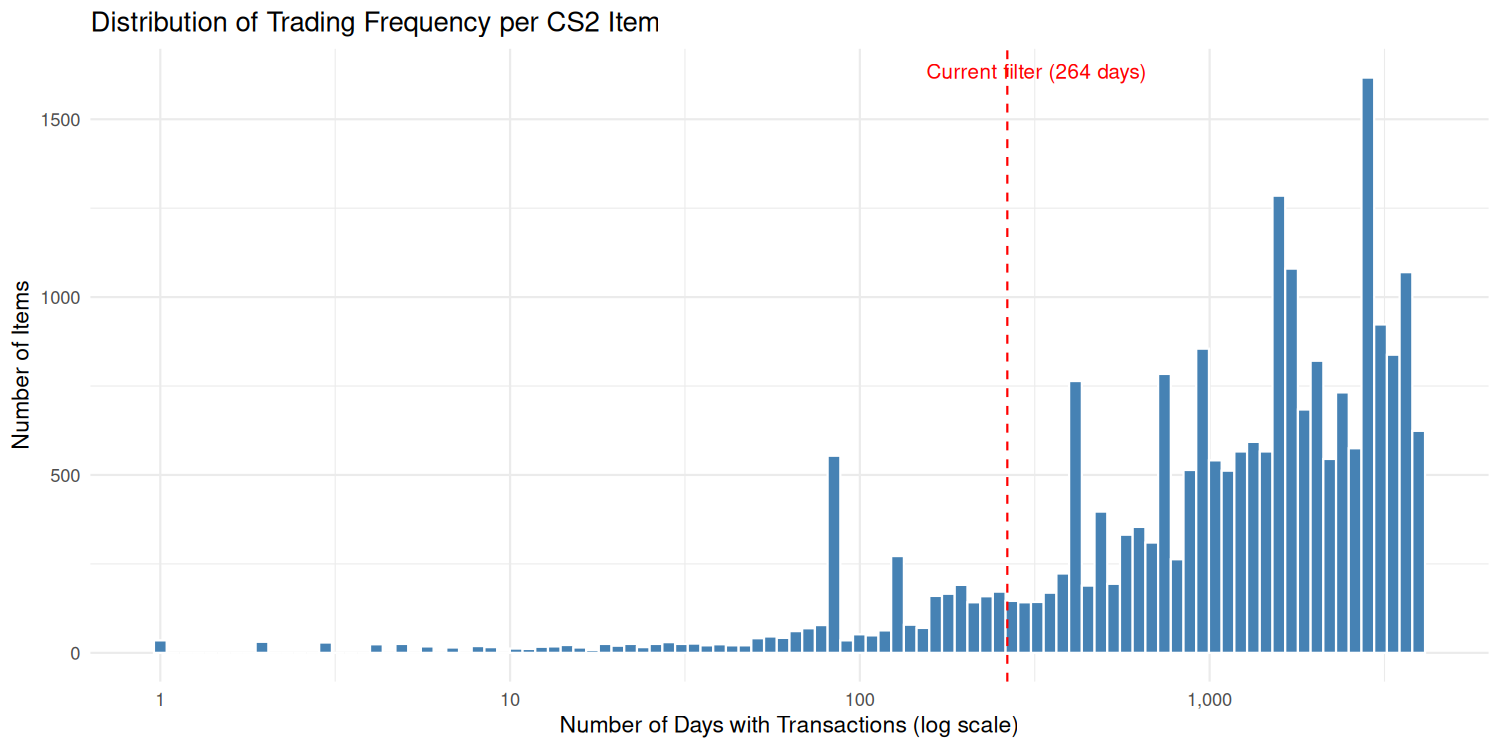
\includegraphics[width=\linewidth]{../images/index/trading_frequency.png}
  \caption{Distribution of trading frequency per CS2 item (number of days with
    at least one recorded transaction).}
  \label{fig:trading_frequency}
\end{figure}

Figure~\ref{fig:trading_frequency} shows the distribution of trading days per
item across the full raw dataset (log scale). The distribution is strongly
right-skewed: a large mass of items trade on very few days and a smaller group
of liquid items trade consistently throughout the sample. The vertical dashed
line marks the current liquidity threshold: items to its left are excluded
because at least one calendar month in their history contains fewer than two
transactions. The retained items (to the right) contribute stable daily price
observations throughout the 3,960-day sample, supporting the reliability of
the value-weighted index.

% ─── A.3 GARCH Diagnostics ───────────────────────────────────────────────────
\subsection{GARCH Diagnostics}

\begin{figure}[H]
  \centering
  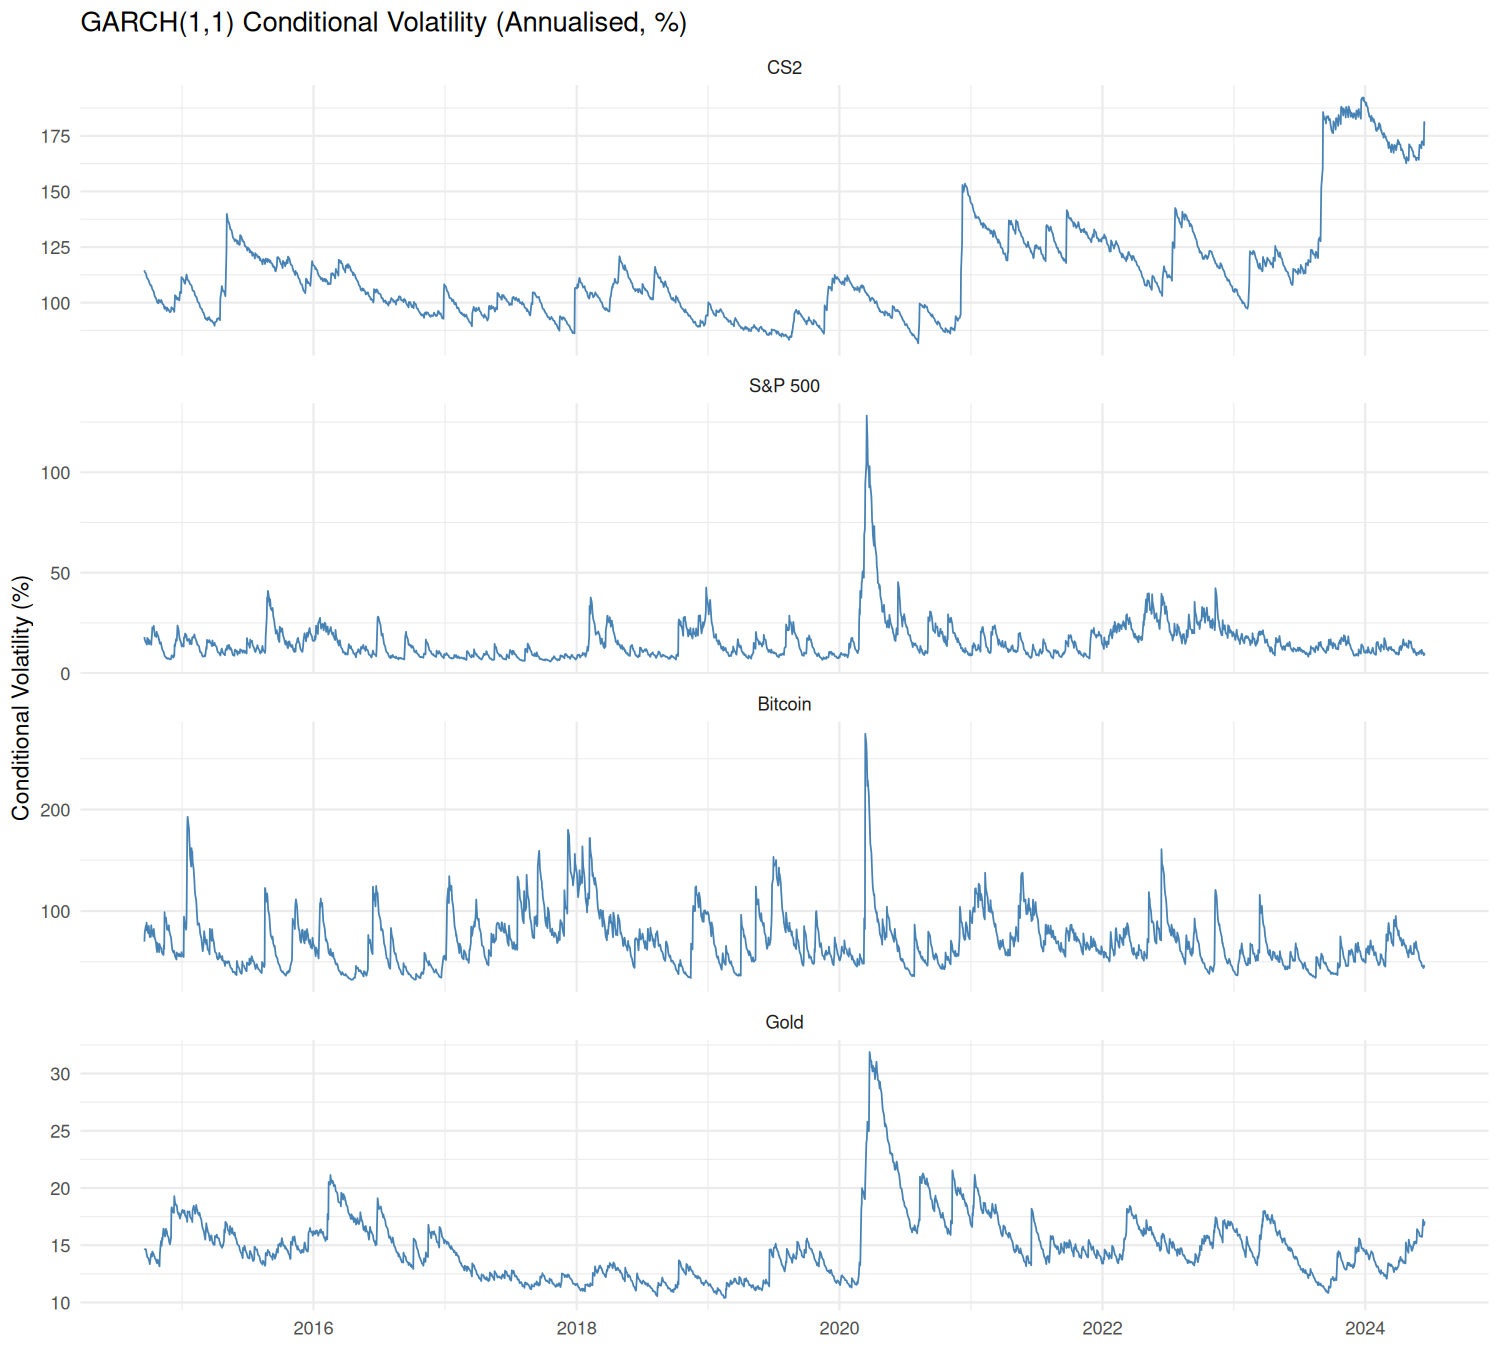
\includegraphics[width=\linewidth]{../images/garch/conditional_volatility.png}
  \caption{GARCH(1,1) conditional volatility (annualised, \%) for all four
    assets, August 2014 to June 2024.}
  \label{fig:cond_vol}
\end{figure}

Figure~\ref{fig:cond_vol} shows the estimated conditional volatility series for
each asset. Several well-known market stress episodes are visible in the
comparison assets: the S\&P~500 spike in March~2020 (COVID-19 shock), the
Bitcoin collapse of November~2022 (FTX bankruptcy), and the gold spike in
March~2022 (Russia--Ukraine war). CS2 exhibits a qualitatively different
profile: elevated volatility tends to persist in multi-month regimes rather than
arriving as discrete spikes. This is consistent with the ARCH coefficient
$\hat{\alpha} = 0.0151$ (far below Bitcoin's 0.1265), which means individual
return shocks transmit only weakly into the next day's conditional variance, and
the GARCH coefficient $\hat{\beta} = 0.9839$, which ensures that whatever
variance level is reached decays extremely slowly. The contrast with Bitcoin
--- which has the same persistence (0.9990) but reacts sharply to individual
shocks --- confirms that the Steam Marketplace's closed trading hours, illiquid
order book, and slow information transmission shape a distinct volatility
microstructure.

\begin{figure}[H]
  \centering
  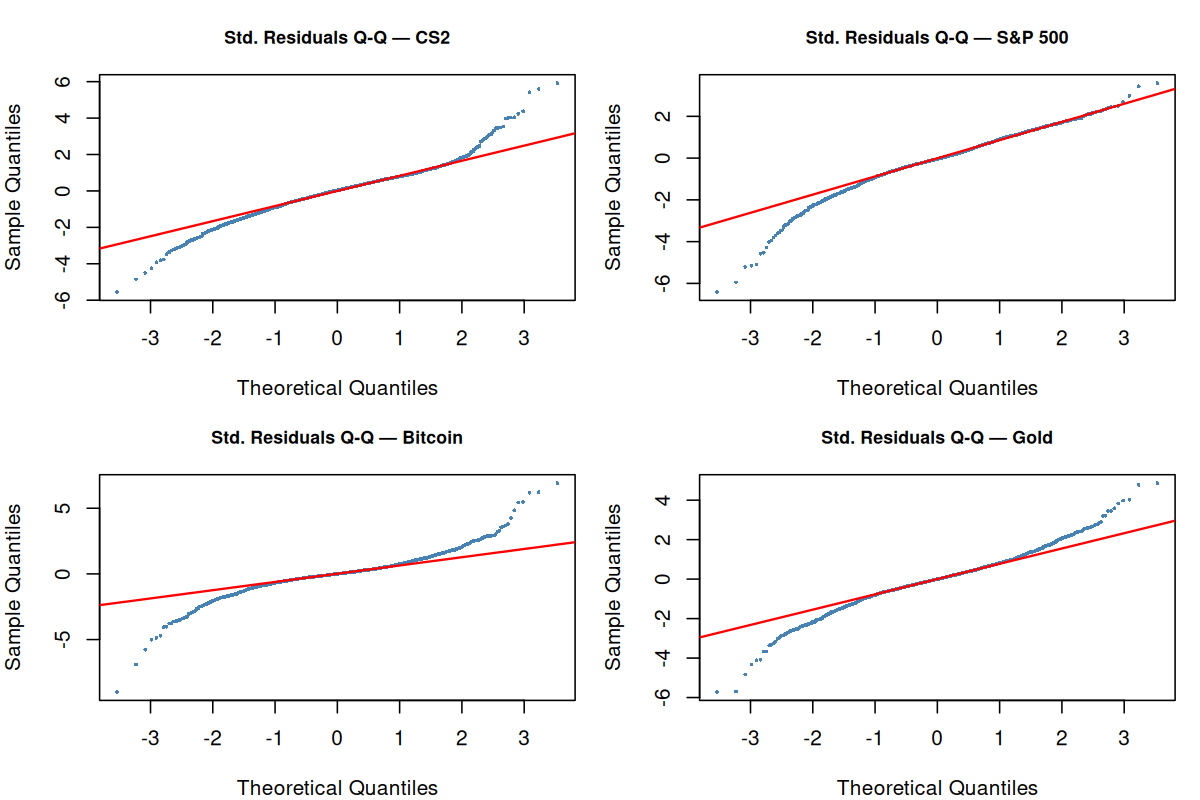
\includegraphics[width=\linewidth]{../images/garch/residual_qq.png}
  \caption{Q-Q plots of standardised GARCH(1,1) residuals against the standard
    normal for all four assets. Systematic tail departures from the diagonal
    motivate the student-$t$ innovation assumption.}
  \label{fig:residual_qq}
\end{figure}

Figure~\ref{fig:residual_qq} plots standardised GARCH(1,1) residuals against
the standard normal quantiles. The plots are not an adequacy check against the
fitted student-$t$ distribution; rather, they serve as a diagnostic showing
\emph{why} the Gaussian assumption is inappropriate and why the student-$t$
specification was chosen. All four assets exhibit systematic heavy-tail
departures (points fan above the upper diagonal and below the lower diagonal),
confirming the fat-tailed nature of standardised residuals. The central mass of
each distribution tracks closely along the diagonal, indicating that
GARCH(1,1) successfully removes the conditional mean structure and that the
residual non-normality is concentrated in the tails, precisely where the
student-$t$ distribution provides additional flexibility relative to the
Gaussian.

% ─── A.4 VAR Diagnostics ─────────────────────────────────────────────────────
\subsection{VAR Diagnostics}

\begin{table}[H]
\centering
\caption{VAR Lag Selection Criteria for Lags 1--10 (lower is better)}
\label{tab:lag_selection}
\begin{tabular}{lrrrr}
\hline
Lag & AIC & HQ & BIC & FPE ($\times 10^{-13}$) \\
\hline
1  & $-29.969$ & $-29.951$ & $-29.921$ & $0.965$ \\
2  & $-30.037$ & $-30.006$ & $-29.952$ & $0.901$ \\
3  & $-30.099$ & $-30.054$ & $-29.976$ & $0.847$ \\
\textbf{4}  & $\mathbf{-30.172}$ & $\mathbf{-30.114}$ & $\mathbf{-30.011}$ & $\mathbf{0.788}$ \\
5  & $-30.184$ & $-30.111$ & $-29.984$ & $0.778$ \\
6  & $-30.190$ & $-30.103$ & $-29.952$ & $0.774$ \\
7  & $-30.207$ & $-30.107$ & $-29.931$ & $0.761$ \\
8  & $-30.222$ & $-30.108$ & $-29.908$ & $0.749$ \\
\textbf{9}  & $-30.234$ & $-30.106$ & $-29.882$ & $0.741$ \\
10 & $-30.231$ & $-30.089$ & $-29.840$ & $0.743$ \\
\hline
\multicolumn{5}{l}{\small Bold row: BIC optimum (p\,=\,4). AIC and FPE optimum: p\,=\,9.}
\end{tabular}
\end{table}

Table~\ref{tab:lag_selection} reports information criteria for lag orders 1--10.
BIC (labelled SC in the \texttt{vars} package) selects $p = 4$, while AIC and
FPE select $p = 9$. The penalty differential between AIC and BIC grows with the
number of parameters, making BIC more conservative in models with a large
endogenous dimension --- here, $4$ variables $\times$ $p$ lags per equation.
The BIC-selected VAR(4) uses $4 \times 4 \times 4 + 4 = 68$ parameters, which
is already a substantial parameterisation for $N = 2{,}444$ effective
observations. The marginal improvement in AIC from lag 4 to lag 9 is modest
(from $-30.172$ to $-30.234$), suggesting that the additional lags capture only
weak dynamics and that the parsimonious BIC choice is appropriate for
inference.

\begin{table}[H]
\centering
\caption{Ljung-Box Residual Autocorrelation Tests --- VAR(4), Lag 10}
\label{tab:ljungbox}
\begin{tabular}{lrrl}
\hline
Asset    & $Q(10)$ & $p$-value & Conclusion \\
\hline
CS2      & 92.11   & $<0.001$  & Residual autocorrelation detected \\
S\&P 500 & 98.26   & $<0.001$  & Residual autocorrelation detected \\
Bitcoin  & 10.36   & $0.410$   & No significant autocorrelation \\
Gold     &  5.78   & $0.833$   & No significant autocorrelation \\
\hline
\end{tabular}
\end{table}

Table~\ref{tab:ljungbox} reports univariate Ljung-Box tests on VAR(4) residuals.
Bitcoin and Gold show no evidence of residual autocorrelation at lag~10
($p > 0.4$), confirming that VAR(4) is adequate for those series. CS2 and the
S\&P~500 exhibit significant residual autocorrelation ($p < 0.001$), indicating
that four lags are insufficient to fully capture the joint dynamics. For CS2,
this is unsurprising given the strong negative first-order autocorrelation in
the raw series (AR coefficient at lag~1: $\hat{\phi}_{11} = -0.485$, $p <
0.001$) and the Steam Marketplace's two-day settlement lag, which imparts a
mechanical negative autocorrelation. For the S\&P~500, weekly seasonality in
trading patterns likely contributes.

These findings have two implications for the main analysis. First, the AIC's
preferred order of $p = 9$ would reduce residual autocorrelation but at the cost
of 80 additional parameters, raising degrees-of-freedom concerns and
multicollinearity risks with $N = 2{,}444$ effective observations. Second, the
Granger causality conclusions are not materially affected: the tests found no
significant predictive power from any benchmark to CS2 or vice versa, and
residual misspecification of this type generally inflates standard errors,
making it harder to reject the null of no causality --- if anything, a
better-specified model would be even less likely to find significance. This
argument addresses test size rather than coefficient bias; a higher-lag VAR or
an ARMA-augmented specification for CS2 would be needed to fully resolve the
residual autocorrelation, and constitutes a natural direction for future
work.

% ─── A.5 R Code ──────────────────────────────────────────────────────────────
\subsection{R Code}

All analysis is implemented in R using \texttt{renv} for reproducible package
management. The pipeline runs sequentially through five scripts; each section
below documents one step. Package dependencies are declared at the top of each
script and installed via \texttt{renv::restore()}.

% ── Step 1 ───────────────────────────────────────────────────────────────────
\subsubsection*{Step 1 --- Data Preprocessing (\texttt{src/01\_data\_preprocessing.R})}

Reads all raw item CSV files exported from the Steam Marketplace, decodes
URL-encoded filenames using a name conversion table, parses structured metadata
(weapon, skin name, wear condition, item category, StatTrak/Souvenir flags),
aggregates intraday records to daily VWAP, and saves the result to
\texttt{data/processed/cs2\_daily.parquet}.

\begin{lstlisting}[style=Rstyle, caption={Step 1: Data preprocessing and daily VWAP aggregation}]
library(data.table); library(arrow); library(here); library(stringr)

ITEMS_DIR  <- here("data", "raw", "items")
NAME_TABLE <- here("data", "raw", "name_conversion_table.csv")
OUT_FILE   <- here("data", "processed", "cs2_daily.parquet")
BATCH_SIZE <- 1000

WEAR_CONDITIONS <- c(
  "Factory New", "Minimal Wear", "Field-Tested", "Well-Worn", "Battle-Scarred"
)

# Name lookup table (URL-encoded -> decoded item names)
name_tbl    <- fread(NAME_TABLE, encoding = "UTF-8")
setnames(name_tbl, c("encoded", "decoded"))
name_lookup <- setNames(name_tbl$decoded, name_tbl$encoded)

# Parse structured metadata from a decoded item name
parse_item_name <- function(decoded_name) {
  name        <- decoded_name
  is_special  <- startsWith(name, "★")
  is_stattrak <- grepl("StatTrak™", name, fixed = TRUE)
  is_souvenir <- grepl("Souvenir",      name, fixed = TRUE)

  name <- sub("^★\\s*", "", name)
  name <- sub("StatTrak™\\s*", "", name)
  name <- sub("Souvenir\\s*", "", name)
  name <- trimws(name)

  wear <- NA_character_
  for (w in WEAR_CONDITIONS) {
    pattern <- paste0("\\s*\\(", w, "\\)$")
    if (grepl(pattern, name)) {
      wear <- w; name <- trimws(sub(pattern, "", name)); break
    }
  }

  parts     <- strsplit(name, " | ", fixed = TRUE)[[1]]
  weapon    <- trimws(parts[1])
  skin_name <- if (length(parts) >= 2) trimws(paste(parts[-1], collapse=" | "))
               else NA_character_

  item_category <- dplyr::case_when(
    grepl("Graffiti",  weapon,       fixed=TRUE) ~ "graffiti",
    grepl("Music Kit", decoded_name, fixed=TRUE) ~ "music_kit",
    grepl("Capsule",   decoded_name, fixed=TRUE) ~ "capsule",
    grepl("Case",      weapon,       fixed=TRUE) ~ "case",
    grepl("Package",   decoded_name, fixed=TRUE) ~ "case",
    grepl("Sticker",   weapon,       fixed=TRUE) ~ "sticker",
    is_special & grepl("Gloves|Wraps|Hand", weapon) ~ "glove",
    is_special                                   ~ "knife",
    !is.na(wear)                                 ~ "weapon_skin",
    TRUE                                         ~ "other"
  )

  base_item <- if (!is.na(skin_name)) paste0(weapon, " | ", skin_name) else weapon
  list(weapon=weapon, skin_name=skin_name, wear=wear, base_item=base_item,
       item_category=item_category, is_stattrak=is_stattrak,
       is_special=is_special, is_souvenir=is_souvenir)
}

# Process one CSV file: decode name, aggregate to daily VWAP, attach metadata
process_file <- function(filepath) {
  enc_name <- tools::file_path_sans_ext(basename(filepath))
  dec_name <- name_lookup[enc_name]
  if (is.na(dec_name)) dec_name <- URLdecode(enc_name)

  dt <- tryCatch(fread(filepath, showProgress=FALSE, select=1:4),
                 error=function(e) NULL)
  if (is.null(dt) || nrow(dt) == 0) return(NULL)
  setnames(dt, c("price", "quantity", "date_str", "unix_ts"))

  dt[, date := as.Date(as.POSIXct(unix_ts, origin="1970-01-01", tz="UTC"))]
  dt <- dt[, .(price    = sum(price * quantity) / sum(quantity),
               quantity = as.integer(sum(quantity))), by = date]

  meta <- parse_item_name(dec_name)
  dt[, `:=`(item_name=dec_name, item_category=meta$item_category,
             weapon=meta$weapon, skin_name=meta$skin_name, wear=meta$wear,
             base_item=meta$base_item, is_stattrak=meta$is_stattrak,
             is_special=meta$is_special, is_souvenir=meta$is_souvenir)]
  dt
}

# Batched processing over all CSV files
files     <- list.files(ITEMS_DIR, pattern="\\.csv$", full.names=TRUE)
n_batches <- ceiling(length(files) / BATCH_SIZE)
batches   <- vector("list", n_batches)

for (b in seq_len(n_batches)) {
  idx        <- ((b-1)*BATCH_SIZE+1):min(b*BATCH_SIZE, length(files))
  batch      <- lapply(files[idx], process_file)
  batches[[b]] <- rbindlist(Filter(Negate(is.null), batch), fill=TRUE)
}

cs2 <- rbindlist(batches, fill=TRUE)
cs2[, trading_value := price * quantity]
setcolorder(cs2, c("date","item_name","item_category","weapon","skin_name",
                   "wear","base_item","is_stattrak","is_special","is_souvenir",
                   "price","quantity","trading_value"))
setorder(cs2, item_name, date)

write_parquet(cs2, OUT_FILE)
\end{lstlisting}

% ── Step 2 ───────────────────────────────────────────────────────────────────
\subsubsection*{Step 2 --- Index Construction (\texttt{src/02\_index\_construction.R})}

Filters to wearable item categories, excludes StatTrak and Souvenir variants,
applies the monthly liquidity filter, and aggregates surviving items into a
daily value-weighted index. Saves the index to
\texttt{data/processed/cs2\_index.parquet} and a filter funnel summary to
\texttt{data/processed/filter\_stats.csv}.

\begin{lstlisting}[style=Rstyle, caption={Step 2: Liquidity filter and value-weighted index construction}]
library(data.table); library(arrow); library(here)

IN_FILE  <- here("data", "processed", "cs2_daily.parquet")
OUT_FILE <- here("data", "processed", "cs2_index.parquet")
WEARABLE_CATS <- c("weapon_skin", "knife", "glove")
LIQUIDITY_MIN <- 2L   # minimum trades per calendar month

cs2 <- as.data.table(read_parquet(IN_FILE))

# Step 1: Restrict to wearables, exclude StatTrak and Souvenir
n_raw_items <- uniqueN(cs2$item_name)
n_raw_base  <- uniqueN(cs2$base_item)

cs2 <- cs2[item_category %in% WEARABLE_CATS & !is_stattrak & !is_souvenir]

n_wear_items <- uniqueN(cs2$item_name)
n_wear_base  <- uniqueN(cs2$base_item)

# Step 2: Liquidity filter - drop any base_item with < 2 trades in any month
cs2[, month := format(date, "%Y-%m")]
monthly  <- cs2[, .(monthly_qty = sum(quantity)), by = .(base_item, month)]
illiquid <- monthly[monthly_qty < LIQUIDITY_MIN, unique(base_item)]
cs2      <- cs2[!base_item %in% illiquid]
cs2[, month := NULL]
n_liquid_base <- uniqueN(cs2$base_item)

# Save filter funnel for appendix table
filter_stats <- data.table(
  Stage = c("Raw items (all categories, all variants)",
            "After wearable categories + StatTrak/Souvenir exclusion",
            "After liquidity filter (>=2 trades/month in every month)"),
  Item_variants = c(n_raw_items, n_wear_items, NA_integer_),
  Base_items    = c(n_raw_base,  n_wear_base,  n_liquid_base)
)
fwrite(filter_stats, here("data", "processed", "filter_stats.csv"))

# Step 3: Value-weighted daily index
# I_t = sum(price_it * qty_it) / sum(qty_it)
index <- cs2[, .(
  index_level  = sum(trading_value) / sum(quantity),
  n_items      = uniqueN(base_item),
  total_volume = sum(quantity)
), by = date]
setorder(index, date)

write_parquet(index, OUT_FILE)
\end{lstlisting}

% ── Step 3 ───────────────────────────────────────────────────────────────────
\subsubsection*{Step 3 --- Exploratory Data Analysis (\texttt{src/03\_eda.R})}

Loads the CS2 index and retrieves S\&P~500, Bitcoin, and Gold prices via
\texttt{quantmod}. Aligns all four series on common trading days, computes
log returns, and produces descriptive statistics, a correlation matrix, ADF
stationarity tests, and all EDA plots. Saves aligned log returns to
\texttt{data/processed/returns.parquet} for downstream scripts.

\begin{lstlisting}[style=Rstyle, caption={Step 3: EDA --- alignment, log returns, statistics, and plots}]
library(data.table); library(arrow); library(here)
library(ggplot2); library(patchwork); library(quantmod); library(tseries)

DATE_FROM <- "2013-08-01"; DATE_TO <- "2024-06-15"

# Load CS2 index
cs2 <- as.data.table(read_parquet(here("data","processed","cs2_index.parquet")))
cs2 <- cs2[, .(date, cs2 = index_level)]

# Download comparison assets
getSymbols(c("^GSPC","BTC-USD","GC=F"), from=DATE_FROM, to=DATE_TO,
           auto.assign=TRUE, warnings=FALSE)
sp500 <- data.table(date=as.Date(index(GSPC)),      sp500=as.numeric(Ad(GSPC)))
btc   <- data.table(date=as.Date(index(`BTC-USD`)), btc  =as.numeric(Ad(`BTC-USD`)))
gold  <- data.table(date=as.Date(index(`GC=F`)),    gold =as.numeric(Cl(`GC=F`)))

# Inner join on common trading days
dt <- Reduce(function(a,b) merge(a,b,by="date"), list(cs2,sp500,btc,gold))
setorder(dt, date)

# Log returns
for (col in c("cs2","sp500","btc","gold"))
  dt[, paste0("r_",col) := c(NA_real_, diff(log(get(col))))]
ret <- dt[!is.na(r_cs2)]

# Descriptive statistics
desc_stats <- function(x) list(
  n=sum(!is.na(x)), mean=mean(x,na.rm=TRUE), sd=sd(x,na.rm=TRUE),
  min=min(x,na.rm=TRUE), max=max(x,na.rm=TRUE),
  skewness=mean(((x-mean(x,na.rm=TRUE))/sd(x,na.rm=TRUE))^3,na.rm=TRUE),
  kurtosis=mean(((x-mean(x,na.rm=TRUE))/sd(x,na.rm=TRUE))^4,na.rm=TRUE)-3
)
stats <- rbindlist(lapply(
  c(cs2="r_cs2",`S&P 500`="r_sp500",Bitcoin="r_btc",Gold="r_gold"),
  function(col) as.data.table(desc_stats(ret[[col]]))), idcol="asset")
print(stats)

# Correlation matrix
cor_mat <- cor(ret[,.(r_cs2,r_sp500,r_btc,r_gold)], use="complete.obs")
rownames(cor_mat) <- colnames(cor_mat) <- c("CS2","S&P 500","Bitcoin","Gold")

# ADF stationarity tests
for (col in c("r_cs2","r_sp500","r_btc","r_gold")) {
  adf <- adf.test(na.omit(ret[[col]]))
  message(sprintf("%-10s  stat=%6.3f  p=%.4f", col, adf$statistic, adf$p.value))
}

theme_set(theme_minimal(base_size=11))

# Figure 1: Normalised price levels (log scale)
levels_long <- melt(dt[, .(date,
  CS2=cs2/cs2[1]*100, `S&P 500`=sp500/sp500[1]*100,
  Bitcoin=btc/btc[1]*100, Gold=gold/gold[1]*100)],
  id.vars="date", variable.name="Asset", value.name="value")
p_levels <- ggplot(levels_long, aes(date,value,colour=Asset)) +
  geom_line(linewidth=0.5) + scale_y_log10() +
  labs(title="Normalised Price Levels (base=100, log scale)",
       x=NULL, y="Index (log scale)", colour=NULL) +
  theme(legend.position="bottom")
ggsave(here("images","eda","levels.png"), p_levels, width=10, height=4, dpi=150)

# Figure 2: Daily log returns
returns_long <- melt(ret[,.(date,CS2=r_cs2,`S&P 500`=r_sp500,
                            Bitcoin=r_btc,Gold=r_gold)],
  id.vars="date", variable.name="Asset", value.name="return")
p_returns <- ggplot(returns_long, aes(date,return)) +
  geom_line(linewidth=0.3, colour="steelblue") +
  facet_wrap(~Asset, ncol=1, scales="free_y") +
  labs(title="Daily Log Returns", x=NULL, y="Log Return")
ggsave(here("images","eda","returns.png"), p_returns, width=10, height=8, dpi=150)

# Figure 3: Correlation heatmap
cor_long <- as.data.table(as.table(cor_mat))
setnames(cor_long, c("Asset1","Asset2","correlation"))
p_cor <- ggplot(cor_long, aes(Asset1,Asset2,fill=correlation)) +
  geom_tile(colour="white") + geom_text(aes(label=round(correlation,2)),size=3.5)+
  scale_fill_gradient2(low="#d73027",mid="white",high="#1a9850",midpoint=0,
                       limits=c(-1,1)) +
  labs(title="Correlation Matrix", x=NULL, y=NULL, fill="r") +
  theme(axis.text.x=element_text(angle=45,hjust=1))
ggsave(here("images","eda","correlation.png"), p_cor, width=5, height=4, dpi=150)

# Figure 4: ACF and PACF of log returns
png(here("images","eda","acf.png"), width=1200, height=800, res=120)
par(mfrow=c(2,4), mar=c(4,4,3,1))
for (col in c("r_cs2","r_sp500","r_btc","r_gold")) {
  label <- switch(col,r_cs2="CS2",r_sp500="S&P 500",r_btc="Bitcoin",r_gold="Gold")
  acf(na.omit(ret[[col]]),  main=paste("ACF -",  label), lag.max=30)
  pacf(na.omit(ret[[col]]), main=paste("PACF -", label), lag.max=30)
}
dev.off()

# Figure 5: Return distributions with normal overlay
norm_curves <- returns_long[, {
  x_seq <- seq(min(return,na.rm=TRUE), max(return,na.rm=TRUE), length.out=300)
  .(x=x_seq, y=dnorm(x_seq, mean(return,na.rm=TRUE), sd(return,na.rm=TRUE)))
}, by=Asset]
p_dist <- ggplot(returns_long, aes(x=return)) +
  geom_histogram(aes(y=after_stat(density)), bins=60,
                 fill="steelblue", colour="white", linewidth=0.1) +
  geom_line(data=norm_curves, aes(x=x,y=y),
            colour="red", linewidth=0.7, inherit.aes=FALSE) +
  facet_wrap(~Asset, scales="free", ncol=2) +
  labs(x="Log return", y="Density",
       title="Return Distributions with Normal Overlay (red)") +
  theme_minimal(base_size=10)
ggsave(here("images","eda","distributions.png"), p_dist, width=8, height=5, dpi=150)

# Save aligned returns for downstream scripts
write_parquet(ret, here("data","processed","returns.parquet"))
\end{lstlisting}

% ── Step 4 ───────────────────────────────────────────────────────────────────
\subsubsection*{Step 4 --- GARCH Volatility Modelling (\texttt{src/04\_garch.R})}

Fits a GARCH(1,1) model with student-$t$ innovations to each of the four return
series using the \texttt{rugarch} package. Extracts and prints the ARCH
coefficient $\hat{\alpha}$, GARCH coefficient $\hat{\beta}$, persistence, and
annualised unconditional volatility. Produces a conditional volatility plot and
a standardised residuals Q-Q diagnostic.

\begin{lstlisting}[style=Rstyle, caption={Step 4: GARCH(1,1) estimation and volatility diagnostics}]
library(data.table); library(arrow); library(here)
library(rugarch); library(ggplot2)

ret <- as.data.table(read_parquet(here("data","processed","returns.parquet")))

ASSETS <- c(CS2="r_cs2", `S&P 500`="r_sp500", Bitcoin="r_btc", Gold="r_gold")

# GARCH(1,1) specification with student-t innovations
spec <- ugarchspec(
  variance.model     = list(model="sGARCH", garchOrder=c(1,1)),
  mean.model         = list(armaOrder=c(0,0), include.mean=TRUE),
  distribution.model = "std"
)

fits <- list(); params <- list()

for (label in names(ASSETS)) {
  x   <- na.omit(ret[[ASSETS[[label]]]])
  fit <- ugarchfit(spec=spec, data=x, solver="hybrid")
  fits[[label]] <- fit

  cf    <- coef(fit)
  alpha <- cf["alpha1"]; beta <- cf["beta1"]; omega <- cf["omega"]
  pers  <- alpha + beta
  uncond_vol_ann <- sqrt(omega / (1 - pers)) * sqrt(252) * 100

  params[[label]] <- data.table(asset=label, omega=omega, alpha=alpha,
    beta=beta, persistence=pers, uncond_vol_ann=uncond_vol_ann)

  message(sprintf("%s: alpha=%.4f  beta=%.4f  persistence=%.4f  vol=%.2f%%",
                  label, alpha, beta, pers, uncond_vol_ann))
}

results <- rbindlist(params)
print(results[, .(asset, alpha=round(alpha,4), beta=round(beta,4),
                  persistence=round(persistence,4),
                  uncond_vol_ann=round(uncond_vol_ann,2))])

# Figure: Conditional volatility (annualised)
vol_dt <- rbindlist(lapply(names(fits), function(label) data.table(
  date  = ret$date[!is.na(ret[[ASSETS[[label]]]])],
  asset = label,
  sigma = as.numeric(sigma(fits[[label]])) * sqrt(252) * 100
)))
vol_dt[, asset := factor(asset, levels=c("CS2","S&P 500","Bitcoin","Gold"))]
p_vol <- ggplot(vol_dt, aes(date,sigma)) +
  geom_line(linewidth=0.4, colour="steelblue") +
  facet_wrap(~asset, ncol=1, scales="free_y") +
  labs(title="GARCH(1,1) Conditional Volatility (Annualised, %)",
       x=NULL, y="Conditional Volatility (%)")
ggsave(here("images","garch","conditional_volatility.png"),
       p_vol, width=10, height=9, dpi=150)

# Figure: Standardised residuals Q-Q plots (motivation for student-t)
png(here("images","garch","residual_qq.png"), width=1200, height=800, res=150)
par(mfrow=c(2,2), mar=c(4,4,3,1))
for (label in names(fits)) {
  std_resid <- as.numeric(residuals(fits[[label]], standardize=TRUE))
  qqnorm(std_resid, main=paste("Std. Residuals Q-Q -", label),
         cex.main=0.85, pch=16, cex=0.4, col="steelblue")
  qqline(std_resid, col="red", lwd=1.5)
}
dev.off()
\end{lstlisting}

% ── Step 5 ───────────────────────────────────────────────────────────────────
\subsubsection*{Step 5 --- VAR and Granger Causality (\texttt{src/05\_var\_granger.R})}

Estimates a VAR($p$) model on the joint system of four log return series using
the \texttt{vars} package. Selects the lag order by BIC via \texttt{VARselect},
runs joint Granger causality F-tests via \texttt{causality()}, and saves
residual diagnostics. The fitted VAR object is saved to
\texttt{data/processed/var\_model.rds} for potential reuse.

\begin{lstlisting}[style=Rstyle, caption={Step 5: VAR lag selection, Granger causality, and residual diagnostics}]
library(data.table); library(arrow); library(here); library(vars)

ret      <- as.data.table(read_parquet(here("data","processed","returns.parquet")))
var_data <- na.omit(ret[, .(r_cs2, r_sp500, r_btc, r_gold)])

# Lag selection: AIC=9, BIC=4 -> use BIC for parsimony
lag_select <- VARselect(var_data, lag.max=10, type="const")
print(lag_select$selection)

lag_table <- as.data.table(t(lag_select$criteria), keep.rownames="Lag")
lag_table[, Lag := as.integer(Lag)]
fwrite(lag_table, here("data","processed","var_lag_selection.csv"))

p <- lag_select$selection["SC(n)"]   # BIC-selected lag order

# Fit VAR(p)
var_model <- VAR(var_data, p=p, type="const")
summary(var_model)

# Granger causality: each variable tested against the entire remaining system
tests <- list(
  "Bitcoin  -> system" = "r_btc",
  "S&P 500  -> system" = "r_sp500",
  "Gold     -> system" = "r_gold",
  "CS2      -> system" = "r_cs2"
)

granger_results <- rbindlist(lapply(names(tests), function(name) {
  res   <- causality(var_model, cause=tests[[name]])
  pval  <- res$Granger$p.value
  fstat <- res$Granger$statistic
  message(sprintf("%-25s  F=%6.3f  p=%.4f", name, fstat, pval))
  data.table(direction=name, F_stat=round(fstat,3), p_value=round(pval,4))
}))
print(granger_results)

saveRDS(var_model, here("data","processed","var_model.rds"))

# Ljung-Box residual autocorrelation tests (lag=10)
resid_mat    <- residuals(var_model)
asset_labels <- c(r_cs2="CS2",r_sp500="S&P 500",r_btc="Bitcoin",r_gold="Gold")

lb_results <- rbindlist(lapply(colnames(resid_mat), function(col) {
  test <- Box.test(resid_mat[, col], lag=10, type="Ljung-Box")
  data.table(Asset=asset_labels[col], Q_stat=round(test$statistic,3),
             p_value=round(test$p.value,4), Df=test$parameter)
}))
print(lb_results)
fwrite(lb_results, here("data","processed","var_ljungbox.csv"))
\end{lstlisting}
